\documentclass[11pt, oneside, a4paper]{article}
%--------This section sets up the document class and packages.
\usepackage[includeheadfoot, margin=20mm, headheight=20mm]{geometry} 
\usepackage{fancyhdr}
\usepackage{mwe}
\usepackage{amsmath}
\usepackage{amsthm}
\usepackage[utf8]{inputenc}
\usepackage{amssymb}
%\usepackage{xcolor,graphicx}
\usepackage{hyperref}
\usepackage{centernot}
\usepackage{tikz}  % Uncomment this line iff you are using the tikz package to add drawings
\usepackage{tkz-euclide}
\usepackage{pgf}
\usepackage{pgfplots}
\pgfplotsset{compat=newest}
\pgfplotsset{plot coordinates/math parser=false}
\usepackage[toc,page]{appendix}
\usepackage{hyperref}
\usepackage{pdfpages}
\usepackage{xargs}                      % Use more than one optional parameter in a new commands
%\usepackage[pdftex,dvipsnames]{xcolor}  % Coloured text etc.
% 
\usepackage[colorinlistoftodos,prependcaption]{todonotes}
\newcommandx{\unsure}[2][1=]{\todo[linecolor=red,backgroundcolor=red!25, size=\small,bordercolor=red,#1]{#2}}
\usepackage{url}
\usepackage[ruled,vlined]{algorithm2e}
\SetKwComment{Comment}{$\triangleright$\ }{}
\usepackage{listings}

\allowdisplaybreaks
\pgfplotsset{soldot/.style={color=blue,only marks,mark=*}} \pgfplotsset{holdot/.style={color=blue,fill=white,only marks,mark=*}}

\usepackage{tocloft}
\renewcommand{\cftsecleader}{\cftdotfill{\cftdotsep}}
\renewcommand\labelenumi{(\roman{enumi})}

%--- This section makes possible customized theorem numbering.
\newtheorem{innercustomgeneric}{\customgenericname}
\providecommand{\customgenericname}{}
\newcommand{\newcustomtheorem}[2]{%
  \newenvironment{#1}[1]
  {%
   \renewcommand\customgenericname{#2}%
   \renewcommand\theinnercustomgeneric{##1}%
   \innercustomgeneric
  }
  {\endinnercustomgeneric}
}
\newcustomtheorem{cthm}{Theorem}
\newcustomtheorem{caxm}{Axiom}
\newcustomtheorem{clem}{Lemma}
\newcustomtheorem{ccor}{Corollary}
\newcustomtheorem{cprop}{Proposition}
\newcustomtheorem{cdefn}{Definition}
\newcustomtheorem{ceg}{Example}
\newcustomtheorem{crmk}{Remark}
\newcustomtheorem{ccus}{}
\newcustomtheorem{cprob}{Problem}

%---The following code sets up the way theorems are typeset and labeled.
\newtheorem{thm}{Theorem}
\newtheorem{lem}[thm]{Lemma}
\newtheorem{cor}[thm]{Corollary}
\newtheorem{prop}[thm]{Proposition}
\theoremstyle{definition}
\newtheorem{defn}[thm]{Definition}
\newtheorem{axm}[thm]{Axiom}
\newtheorem{eg}[thm]{Example}
\theoremstyle{remark}
\newtheorem{rmk}[thm]{Remark}
\newtheorem{sol}{Solution}

% \numberwithin{equation}{subsection}
% \numberwithin{thm}{section}

% \newtheorem*{thm}{Theorem}
% \newtheorem*{lem}{Lemma}
% \newtheorem*{cor}{Corollary}
% \newtheorem*{prop}{Proposition}
% \theoremstyle{definition}
% \newtheorem*{defn}{Definition}
% \newtheorem*{axm}{Axiom}
% \newtheorem*{eg}{Example}
% \theoremstyle{remark}
% \newtheorem*{rmk}{Remark}
% \newtheorem*{sol}{Solution}


%---The following code defines a few extra commands that will be useful in some exercises.
\newcommand{\abs}[1]{\lvert#1\rvert}     % Absolute value symbol
\newcommand{\Abs}[1]{\Bigg\lvert#1\Bigg\rvert}     % Absolute value symbol (big)
\newcommand{\Z}{\mathbb Z}              % The set of integers
\newcommand{\Q}{\mathbb Q}              % The set of rationals
\newcommand{\R}{\mathbb R}              % The set of reals
\newcommand{\N}{\mathbb N}              % The set of natural numbers
\newcommand{\C}{\mathbb C}              % The set of complex numbers
\newcommand{\F}{\mathbb F}  

\newcommand{\ZZ}{\mathcal{Z}}
\newcommand{\OO}{\mathcal{O}}
\newcommand{\CC}{\mathcal{C}}
\newcommand{\UU}{\mathcal{U}}
\newcommand{\power}{\mathcal{P}}         % The power set of a set
\newcommand{\bfun}{\mathcal{F}}          % The finite subsets
\newcommand{\Id}{\mathrm{Id}}            % The identity function
\newcommand{\nil}{\emptyset}             % Empty set
\newcommand{\inflim}[1]{\lim_{#1\to\infty}} % Limit to infinity
\newcommand{\ninflim}[1]{\lim_{#1\to\infty}}% Limit to negative infinity
\providecommand{\BVec}[1]{\mathbf{#1}}   % Bold font for vectors
\DeclareMathOperator{\gon}{gon}          % A polygon
\DeclareMathOperator{\Fun}{Fun}          % The set of all functions from one set to another
\DeclareMathOperator{\Perm}{Perm}        % The set of all permutations on a set
\DeclareMathOperator{\Int}{int} %interior of a set
\DeclareMathOperator{\cl}{cl} %closure of a set
\DeclareMathOperator{\diam}{diam}
\DeclareMathOperator{\sinc}{sinc}
\DeclareMathOperator{\rank}{rank}
\DeclareMathOperator{\Span}{span}
\DeclareMathOperator{\len}{length}
%\newcommand{\Re}{\mathrm{Re}} %real part

\providecommand{\LIN}[1]{{\color{blue}#1}} %Linda's notes

% Dave's macros
\definecolor{colorDAS}{RGB}{255,127,0}
\providecommand{\DAS}[1]{{\color{colorDAS}#1}}     % Dave's comments

\usepackage[english]{babel}
\usepackage[utf8]{inputenc}
\usepackage{amsmath}
\usepackage{graphicx}
%\usepackage{physics}
%\usepackage{float}
\usepackage[margin=1.in]{geometry}
\usepackage{tocloft}
\renewcommand{\cfttoctitlefont}{\hfill\Large\bfseries}
\renewcommand{\cftaftertoctitle}{\hfill\hfill}
\renewcommand{\cftloftitlefont}{\hfill\Large\bfseries}
\renewcommand{\cftafterloftitle}{\hfill}
\renewcommand{\cftlottitlefont}{\hfill\Large\bfseries}
\renewcommand{\cftafterlottitle}{\hfill}
% These 6 lines will center the titles of the table of contents, list of figures and list of tables
% --------------------------------------------------------------------------
\begin{document}

\begin{titlepage}
\pagenumbering{gobble}
% \addcontentsline{toc}{section}{Abstract}
\begin{center}
\vspace{1cm}
\huge
\textbf{Algorithmic Solution of\\ High Order Partial Differential Equations\\
in Julia\\ via the Fokas Transform Method}

\LARGE
\vspace{.5cm}
An Initial Thesis Presented in Partial Fulfillment of\\ the Honours Bachelor's Degree in Science\\
\vspace{.5cm}
\textbf{Linfan Xiao}\\
\vspace{.5cm}
\Large
\vspace{.5cm}
\Large
% \textbf{Abstract}
\end{center}
% TBD

\vfill
\begin{center}	
Mathematical, Computational, and Statistical Sciences\\
Under the supervision of Prof. Dave Smith\\
Yale-NUS College\\
March 2019\\
\end{center}
\end{titlepage}
\pagenumbering{gobble}
\tableofcontents
\listoffigures
\listoftables
\pagebreak
\pagenumbering{gobble}
% \begin{center}\section*{Acknowledgments}\end{center}
% \addcontentsline{toc}{section}{Acknowledgments}
% TBD

\pagebreak
\pagenumbering{arabic}

\section{Introduction}
Evolution partial differential equations (PDEs) relate a quantity to its rates of change with respect to both time and position. Evolution PDEs can model a variety of phenomena in physics, such as wave propagation and particle motion. This project concerns implementing an algorithmic procedure to solve a certain class of initial-boundary value problems (IBVP) for evolution PDEs in the finite interval \cite{Smith2016} based on the Fokas transform method \cite{Fokas2008}. The implementation is based in Julia, with a focus on symbolic results among numeric features.

\subsection{Motivation}
To motivate the project, suppose we want to solve some IBVPs.

Certain IBVPs (henceforth referred to as type I problems) can be solved algorithmically via classical transform pairs such as the Fourier transform (Figure \ref{fig:classical_transform}). For example, the heat equation
\[\frac{\partial}{\partial t}u = a\frac{\partial}{\partial x^2}u,\quad -\infty<x<\infty\]
with initial condition $u(x,0) = u_0(x)$ can be solved by \textbf{TBD}
\begin{figure}[htpb!]
    \centering
    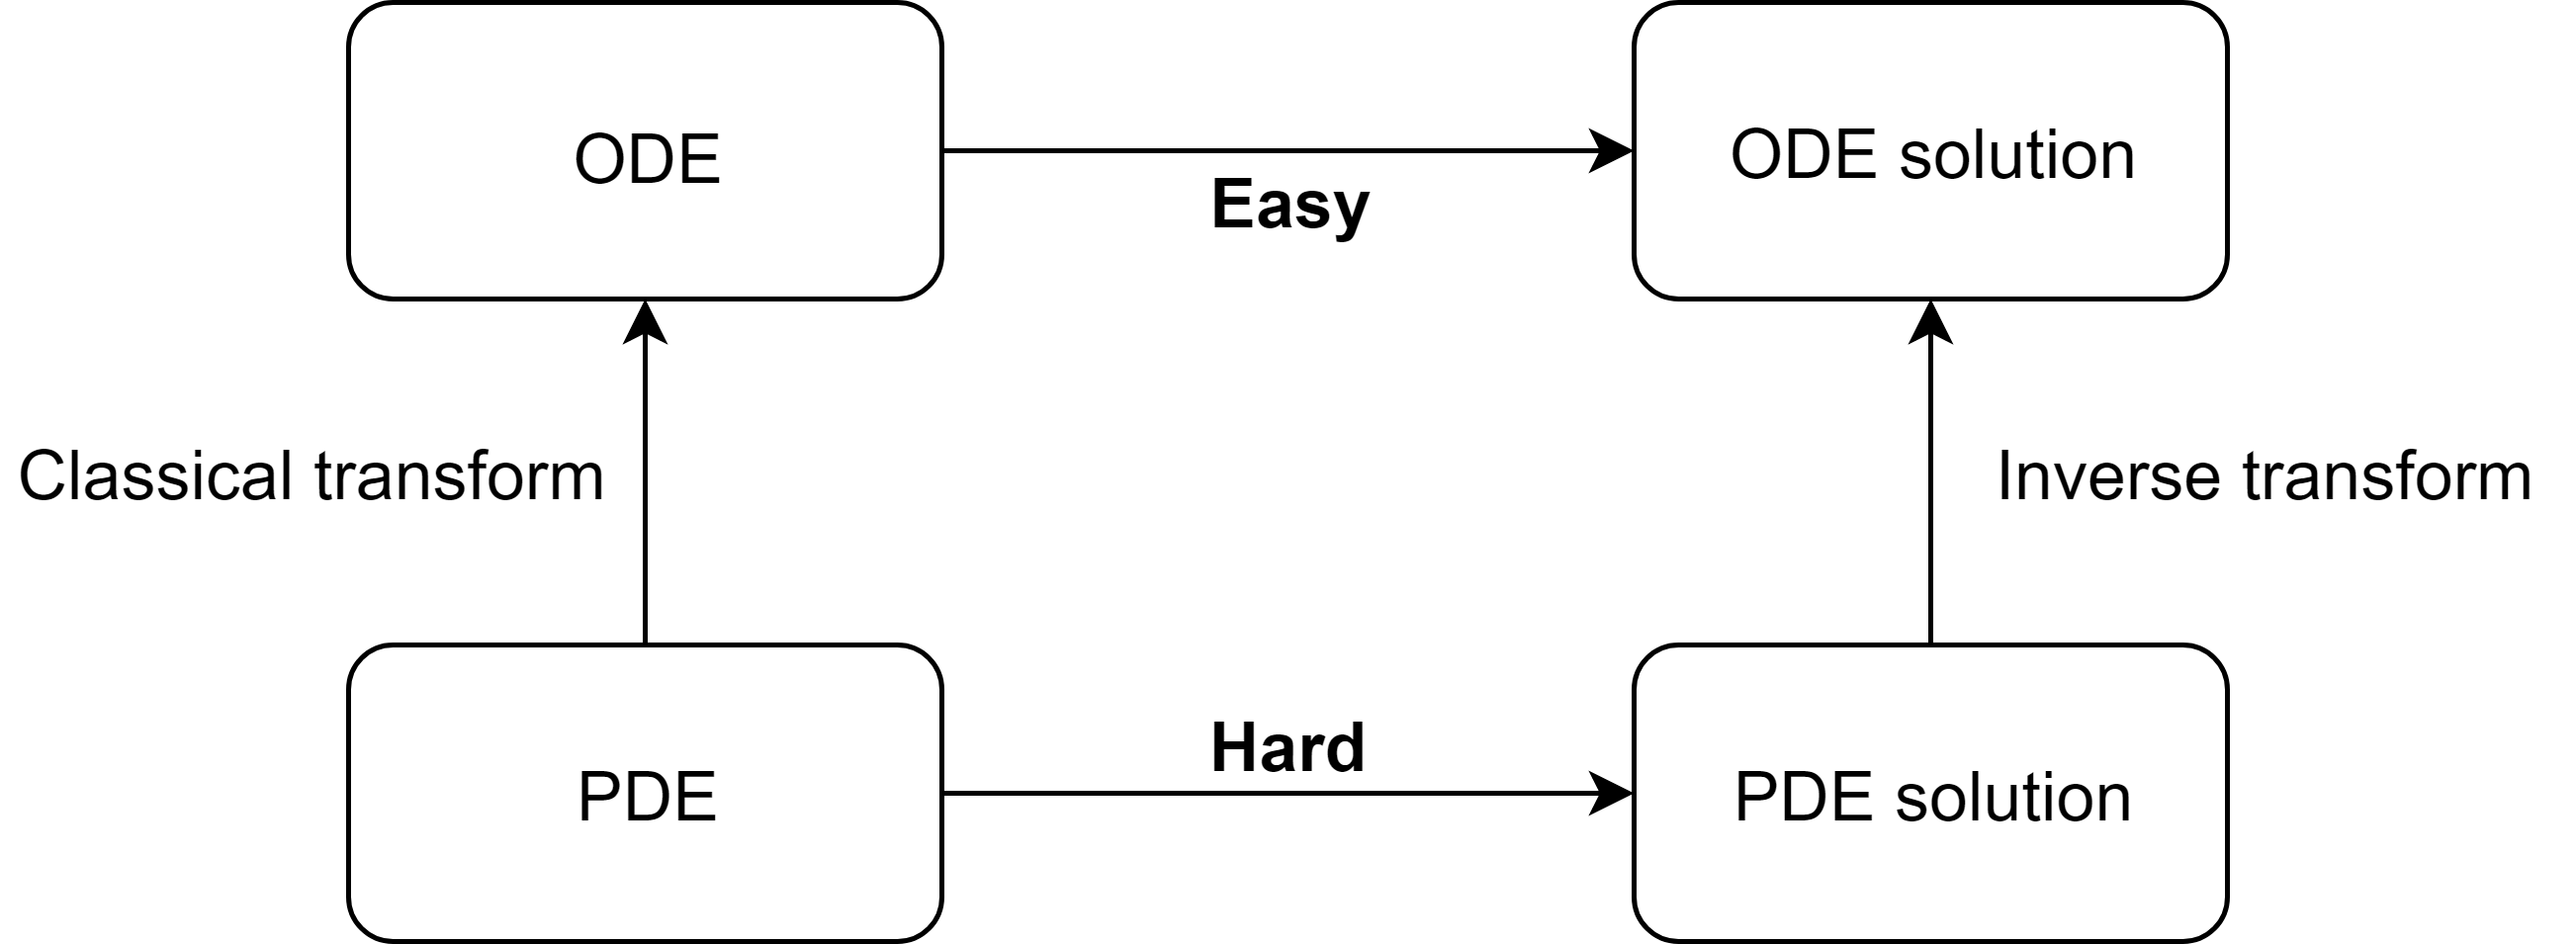
\includegraphics[width=0.8\textwidth]{classical_transform.png}
    \caption{Solving type I IBVPs using classical transform pairs.}
    \label{fig:classical_transform}
\end{figure}

For more complicated IBVPs (henceforth referred to as type II problems), however, no such classical transform pairs exist. In fact, solving these IBVPs typically requires a combination of ad-hoc methods. These methods are often specific to the given problem and cannot be generalized to problems with different parameters (e.g., IBVP involving PDE of a different order or different boundary conditions).

The Fokas transform method \cite{Fokas2008} extends the idea of transform pairs to solving type II problems by constructing non-classical transform pairs based on the problem parameters. Since appropriate transform pairs can now be ``customized'' for IBVPs with different parameters, this means that the Fokas method allows solving an entire class of IBVPs algorithmically in a manner similar to Figure \ref{fig:classical_transform} (Figure \ref{fig:non-classical_transform}).
\begin{figure}[htpb!]
    \centering
    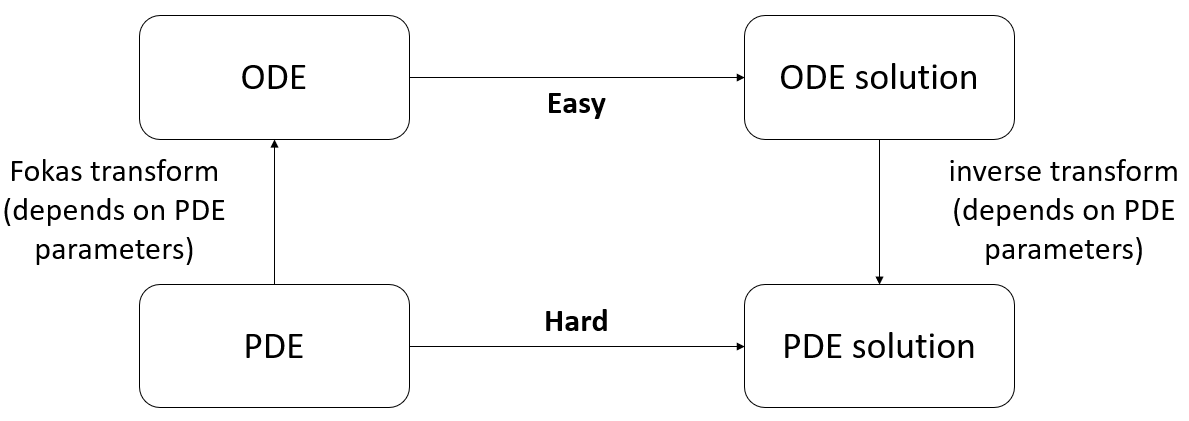
\includegraphics[width=0.8\textwidth]{non-classical_transform.png}
    \caption{Solving type II IBVPs using non-classical transform pairs.}
    \label{fig:non-classical_transform}
\end{figure}

\noindent Examples of IBVPs that can be solved by the Fokas method include second order PDEs of the form
\[\frac{\partial}{\partial t} q(x,t) + a(-i)^2 \frac{\partial^2}{\partial x^2} q(x,t) = 0,\]
with boundary conditions
\begin{equation}\label{eqn:informal_example}
    \begin{split}
    q(0,t) + c_0q(1,t) &= 0\\
    q'(0,t) + c_1q'(1,t) &= 0,
    \end{split}
\end{equation}
or
\begin{align*}
    q(0,t) + c_0 q'(0,t) &= 0\\
    q(1) + c_1 q'(1,t) &= 0,
\end{align*}
where $c_0, c_1\in\hat{\C}:=\C\cup\{0,\infty\}$ (in the sense that if $c_0=\infty$ in \ref{eqn:informal_example}, then dividing by $c_0$ makes $q(0,t)$ disappear and leaves the first equation as $q(1,t) = 0$), as well as third order PDEs of the form 
\[\frac{\partial}{\partial t} q(x,t) \pm i(-i)^2 \frac{\partial^3}{\partial x^3} q(x,t) = 0,\]
with boundary conditions
\begin{align*}
    q(0,t) + c_0 q(1,t) &= 0\\
    q'(0,t) + c_1 q'(1,t) &= 0\\
    q''(0,t) + c_2 q''(1,t) &= 0,
\end{align*}
where $c_j\in\hat{\C}$ for $j=0,1,2$, or 
\begin{align*}
    q(0,t) &= 0\\
    q(1,t) &= 0\\
    q'(0,t) + c q'(1,t) &= 0,
\end{align*}
where $c\in\hat{\C}$. 

In fact, as we will see later, the Fokas method is applicable to IBVPs in the above form with PDEs of any general order $n$. In general, compared to PDEs of higher orders, first and second order PDEs are studied and applied more frequently. The Fokas method advances the understanding of PDEs with higher orders by providing an algorithmic way to solve an entire class of IBVPs of arbitrary order. Using the Fokas method by hand, however, is laborious. It is thus of interest to implement the Fokas method as a software package that aims to supply as much computer aid as possible in the computation process. To our knowledge, despite the presence of various solvers in mathematical softwares such as Mathematica and Matlab, this would be the first time that the Fokas method is implemented. 

In this project, the Fokas method is implemented in Julia, a free open-source, high-performance language for numerical computing \cite{julia}. We choose Julia to be the language of implementation for its support for high-performance numerical computing as well as its open-source property. Commercial softwares may provide access to sophisticated computational algorithms; yet due to being closed-source, there exists a lack of transparency which limits users' understanding of the nature of the software output. Therefore, the mathematical community is moving towards open-source languages like Julia, which allows users to verify the correctness of the output.

As mentioned before, the purpose of implementing the Fokas method in Julia is to 

\subsection{The Initial-Boundary Value Problem}
To formally characterize the class of IBVPs that can be solved by the Fokas method \cite[p.9]{Smith2016}, we first introduce the following definitions.
\begin{itemize}
    \item Define linearly independent boundary forms $B_j: C^\infty[0,1]\to \C$ (where $C^\infty[0,1]$ denotes the class of real-valued functions differentiable for all orders on $[0,1]$) by
    \[B_j\phi := \sum_{k=0}^{n-1}\left(b_{jk}\phi^{(k)}(0) + \beta_{jk}\phi^{(k)}(1)\right),\, j\in\{1,2,\ldots,n\}\]
    where the boundary coefficients $b_{jk}$, $\beta_{jk}\in\R$. 
    \item Define
    \[\Phi:=\{\phi\in C^\infty[0,1]:\, B_j\phi = 0\,\forall j\in\{1,2,\ldots,n\}\}\]
    to be the set of smooth functions $\phi$ satisfying the homogeneous boundary conditions $B_j\phi=0$ for $j\in\{1,2,\ldots,n\}$.
    \item Define 
    \[S = (-i)^n \frac{d^n}{dx^n}\]
    to be a spatial differential operator of order $n$ (i.e., a differential operator in the spatial variable $x$).
\end{itemize}

The Fokas method allows solving any well-posed IBVP that can be written as
\begin{alignat}{3}
    (\partial_t + aS)q(x,t) &= 0\quad &\forall (x,t)&\in (0,1)\times (0,T) \label{eqn:PDE}\\
    q(x,0) &= q_0(x)\in \Phi\quad &\forall x&\in [0,1]\label{eqn:initial_condition}\\
    q(\cdot, t) &= f \in \Phi \quad &\forall t&\in [0,T],\label{eqn:boundary_condition}
\end{alignat}
where $a$ is a complex constant. For the IBVP to be well-posed, we require that $a=\pm i$ if $n$ is odd and $\real(a)\geq 0$ if $n$ is even. Equation \ref{eqn:PDE} is a PDE relating a quantity $q$ to its temporal and spatial rates of change $\partial_t[q]$ and $aS[q]$. \ref{eqn:initial_condition} is the initial condition where the temporal variable $t=0$. \ref{eqn:boundary_condition} corresponds to the homogeneous spatial boundary conditions. 
An example of such IBVPs is the linear Schr\"{o}dinger equation \cite{Taylor2018}, which describes the wave form of a quantum system in free space. The linear Schr\"{o}dinger equation with zero potential is given by
\[ih\frac{\partial w}{\partial t} + \frac{h^2}{2m}\frac{\partial^2 w}{\partial x^2} = 0,\]
where $w(x,t)$ is the wave function, $h$ is the Planck's constant, $m$ is the mass of the particle, and $kx$ describes the potential energy of the particle in the force field. It can be written in the form of \ref{eqn:PDE} as
\[(\partial_t + aS)q(x,t) = 0\]
where $q=w$, $\displaystyle S = \frac{\partial^2}{\partial x^2}$, and $\displaystyle a = \frac{h}{2mi}$. The initial condition 
\[w(x,0) = w_0(x)\]
would mean that the system's wave form at initial stage is described by the wave function $w_0(x)$, and the boundary conditions 
\[w(\cdot, t) = f\]
would mean that the behaviour of the system at its boundary is described by the function $f$ (e.g., if we are considering particles moving in a box, $f$ would describe how the particles behave at the box's boundaries).

For appropriate transform pair $f(x)=f_x(F)$ and $F(\lambda)=F_\lambda(f)$ found using the Fokas method, the solution to the IBVP characterized above is given by \cite[p.15]{Smith2016}
\begin{equation}\label{eqn:solution}
    q(x,t) = f_x(e^{-a\lambda^n t}F_\lambda(f)).
\end{equation}

In the following sections, we first introduce the preliminary definitions and results 

\section{Preliminaries}
We now introduce 

\subsection{Boundary Value Problems and Adjoint Boundary Value Problems}
\subsection{Roots of Exponential Polynomials}
\subsection{The Fokas Transform Pair}

\section{Algorithm}
\subsection{Constructing the Adjoint of a Homogeneous Boundary Condition}
\subsection{Approximating the Roots of an Exponential Polynomial on a Bounded Region}
\subsection{Solving the Initial-Boundary-Value Problem}

\section{Implementation}
\subsection{Platform}
\subsection{Examples}

\pagebreak
\pagenumbering{gobble}
\addcontentsline{toc}{section}{References}

\newpage
\bibliographystyle{unsrt}
\bibliography{C:/Bibtex/Capstone}
\end{document}

